\chapter{Materiais e Métodos}\label{cap:materiais-e-metodos}

Neste capítulo são descritos os materiais e os métodos utilizados no planejamento e no desenvolvimento do trabalho. O conteúdo está estruturado em duas partes: a primeira aborda os materiais empregados, e a segunda apresenta os procedimentos adotados nas etapas de elaboração e execução.


\section{Materiais}\label{sec:materiais}

Na presente seção são apresentadas as tecnologias utilizadas na refatoração e na implementação de novas funcionalidades do E-Museu, sendo elas:


\subsection{\acrshort{php}}

\acrfull{php} é uma linguagem de programação desenvolvida e mantida por uma ampla comunidade de desenvolvedores \textit{open source}, amplamente utilizada no desenvolvimento de aplicações, especialmente no lado do servidor, sendo capaz de gerar conteúdo dinâmico para a \textit{World Wide Web}. Neste trabalho, o \acrshort{php} permaneceu como linguagem principal do \textit{back-end}, adotando-se a série 8.5 compatível com as dependências do repositório \cite{php}.

    
\subsection{\textit{Laravel}}

O \textit{Laravel} é um conjunto de ferramentas desenvolvidas em \acrshort{php} que tem como objetivo facilitar o desenvolvimento de aplicações web, tornando tarefas complexas mais simples de realizar, manter e atualizar, além de oferecer mais segurança. No projeto, a linha anterior utilizava versão mais antiga do \textit{framework}; ao longo do trabalho, o código foi migrado para a linha major compatível com PHP~8.5 declarada no repositório (Laravel na série~13), visando segurança atualizada e estrutura de projeto alinhada às convenções atuais do \textit{framework} \cite{laravel}.

\subsection{\textit{MySQL}}

O \textit{MySQL} é um sistema de gerenciamento de banco de dados relacional, amplamente utilizado no desenvolvimento de aplicações web, que permite o armazenamento, consulta e manipulação de dados de forma eficiente e segura \cite{mysql}. No projeto, o \textit{MySQL} foi mantido para gerenciar as informações do E-Museu, garantindo integridade e desempenho nas operações do catálogo.


\subsection{\textit{Docker e Docker Compose}}

O \textit{Docker} é uma plataforma que permite criar e executar aplicações em ambientes independentes, garantindo isolamento, portabilidade e consistência entre diferentes ambientes de desenvolvimento e produção \cite{docker}. O \textit{Docker Compose} complementa o \textit{Docker}, permitindo coordenar múltiplos desses ambientes de forma simples, utilizando arquivos de configuração. No projeto, essas ferramentas foram utilizadas para organizar e gerenciar os serviços de aplicação e de dados (incluindo \textit{PHP}, \textit{Laravel} e \textit{MySQL}), com ficheiros distintos para desenvolvimento local, homologação e produção \cite{docker,dockercompose}.


\subsection{\textit{Git}}

O \textit{Git} é a principal ferramenta de controle de versões, utilizada para registrar alterações, organizar, compartilhar e gerenciar o código-fonte de projetos de forma eficiente entre desenvolvedores \cite{git}.


\subsection{\textit{GitHub}}
    
O \textit{GitHub} é uma plataforma online integrada ao \textit{Git}, que permite o armazenamento e o compartilhamento de códigos-fonte. Oferece recursos como \textit{pull requests}, \textit{issues}, \textit{projects} e ferramentas de automação, como \acrfull{ci/cd}, que auxiliam na organização, no controle de versão e na documentação dos projetos \cite{github}.


\subsection{\textit{Coolify} e \textit{CapRover}} 

O \textit{Coolify} é uma plataforma de \textit{deploy} e gerenciamento de aplicações que simplifica a hospedagem de sistemas em servidores próprios ou em nuvem \cite{coolify, caprover, nixpacks}. Ela oferece uma interface intuitiva e suporte nativo a containers Docker, possibilitando configurar e monitorar aplicações, bancos de dados e variáveis de ambiente de forma automatizada e segura. No projeto, o \textit{Coolify} foi utilizado para implantar e gerenciar o sistema do E-Museu no servidor da \acrshort{utfpr}, tornando o processo de atualização e manutenção mais ágil e confiável.

Como alternativa, o \textit{CapRover} também foi avaliado por oferecer funcionalidades semelhantes de automação de \textit{deploy} e administração de serviços web. No entanto, optou-se pelo uso do \textit{Coolify} por apresentar vantagens importantes, como suporte nativo ao Docker Compose, uso de Nixpacks - uma ferramenta que identifica automaticamente o tipo de projeto e prepara o ambiente necessário para sua execução, além de contar com gestão integrada de projetos, usuários e permissões, uma comunidade mais ativa, documentação mais completa e melhor integração com o GitHub, que permite automatizar \textit{deploys} de forma mais simples e direta. Já o \textit{CapRover} depende de Dockerfiles manuais e de webhooks configurados para automação.



\section{Métodos}\label{sec:metodos}

Nesta seção são apresentados, em ordem cronológica, os procedimentos adotados nas etapas de elaboração e execução deste Trabalho de Conclusão de Curso.


\subsection{Levantamento de requisitos}

O levantamento de requisitos é a etapa responsável por definir o que será desenvolvido e o que se espera de qualquer projeto. Trata-se de uma fase que exige muita atenção, pois um levantamento impreciso pode comprometer diretamente a qualidade e a precisão do produto final. No caso do E-Museu, essa etapa mostrou-se essencial, sendo amplamente discutida com os professores para garantir o alinhamento entre as necessidades reais e as funcionalidades e refatorações a serem implementadas no sistema.


\subsection{Priorização \acrshort{moscow}}

\acrfull{moscow} é uma técnica de priorização de requisitos em projetos, amplamente utilizada no contexto do desenvolvimento de software, que consiste na divisão dos requisitos em quatro ou cinco categorias distintas, dependendo da preferência \cite{moscow}: 

\begin{itemize}
    \item \textit{Must-have} (deve ter): requisitos essenciais e obrigatórios para o funcionamento mínimo do sistema. Sem eles, o projeto é considerado inviável;
    \item \textit{Should-have} (deveria ter): requisitos importantes, mas não críticos. Sua ausência pode ser contornada temporariamente, sem comprometer o funcionamento básico;
    \item \textit{Could-have} (poderia ter): requisitos desejáveis que agregam valor; porém, a implementação pode ser adiada ou descartada se houver limitação de tempo ou recursos;
    \item \textit{Won't-have} (não terá): requisitos que foram deliberadamente deixados de fora do escopo atual, mas que podem ser considerados em versões futuras do projeto;
    \item \textit{Wish} (desejar): categoria adicional usada em algumas variações da técnica para representar ideias ou funcionalidades que não fazem parte do planejamento atual, mas refletem desejos ou possibilidades futuras.
\end{itemize}

Essa técnica auxilia as equipes a gerenciar o escopo e as expectativas de entrega, garantindo que os esforços sejam concentrados nos aspectos mais críticos e de maior valor para o projeto. A necessidade da utilização desse método surgiu após o levantamento de requisitos do projeto, ou seja, quais requisitos seriam prioridade ou não.   


\subsection{Criar padrão de \textit{Gitflow}}

O \textit{Gitflow} é um modelo de ramificação (\textit{branching model}) que define uma estrutura organizada para o uso do \textit{Git} durante o desenvolvimento de um projeto \cite{gitdocs, githubdocs}. Ele propõe um fluxo de trabalho padronizado, com regras claras sobre como e quando criar, mesclar e remover \textit{branches}, facilitando o controle de versões, a colaboração entre desenvolvedores e a entrega contínua de novas funcionalidades. Nesse modelo, o desenvolvimento principal é dividido entre dois ramos estáveis:

\begin{itemize}
    \item O \texttt{main}, que representa o código em produção;
    \item E o \texttt{develop}, que concentra o código em desenvolvimento.
\end{itemize}

\noindent A partir deles, são criados ramos auxiliares para diferentes propósitos:

\begin{itemize}
    \item \texttt{work/}: originalmente chamada de \textit{feature}, é o ambiente onde são criadas \textit{branches} específicas para cada tipo de tarefa no desenvolvimento;
    \item \texttt{release/}: para preparar versões estáveis antes do lançamento;
    \item \texttt{hotfix/}: para correções urgentes diretamente na versão em produção.
\end{itemize}

A Figura \ref{fig:gitflow} ilustra os ramos do \textit{GitFlow} mencionados acima.

\begin{figure}[H]
    \centering
    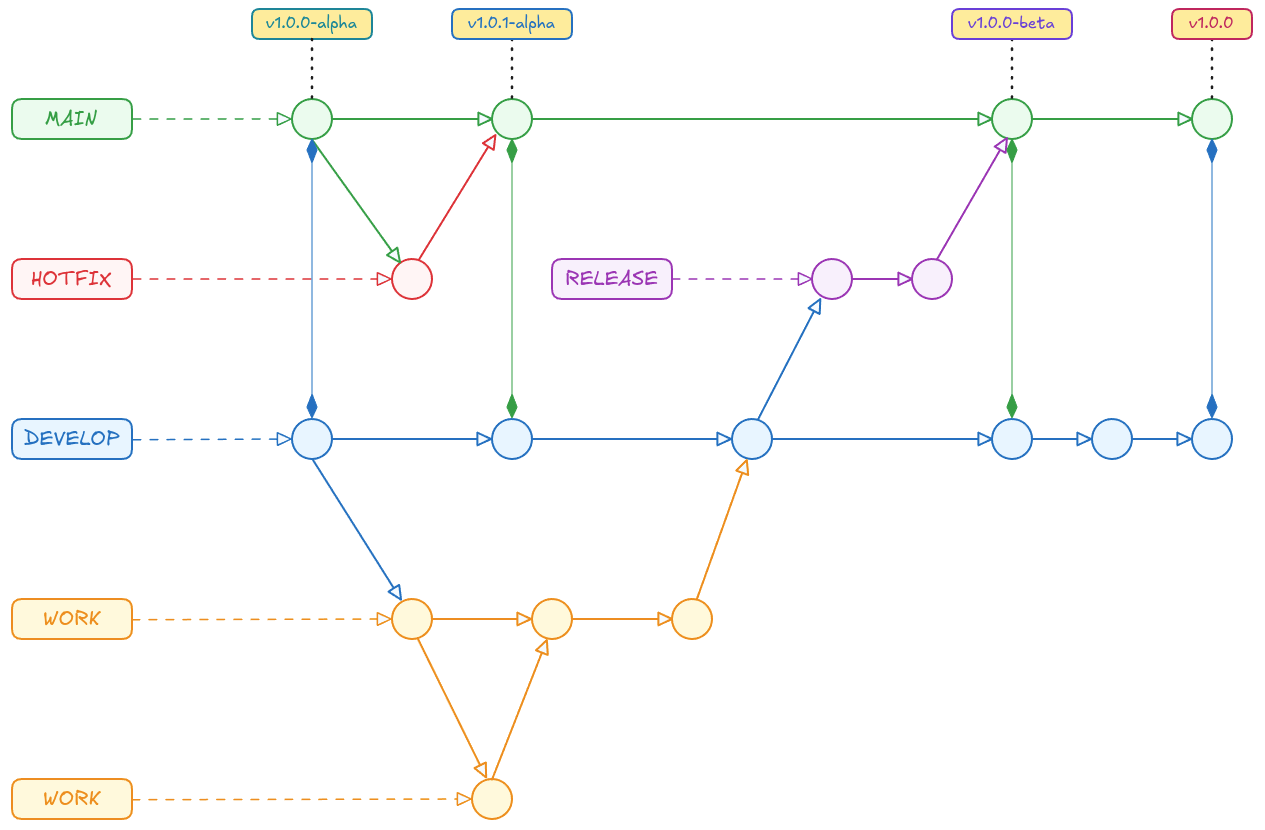
\includegraphics[width=\textwidth]{figuras/gitflow-branches.png}
    \caption{Fluxo de branches no GitFlow.}
    \label{fig:gitflow}
    \caption*{\textbf{Fonte:} Adaptação do padrão GitFlow, com representação desenvolvida por mim.}
\end{figure}

Dessa forma, o \textit{Gitflow} estabelece um ciclo de vida bem definido para cada etapa do projeto, reduzindo conflitos de código e aumentando a rastreabilidade das mudanças.

No contexto do projeto, a padronização inclui a definição de convenções para nomes de \textit{branches} (como \texttt{feature/atividade}), mensagens de \textit{commit} claras e descritivas, regras para abertura de \textit{pull requests} e um fluxo de revisão colaborativo. Essa organização contribui para um desenvolvimento mais coeso, rastreável e escalável.


\subsection{Preparação de ambiente na máquina física na UTFPR para \textit{deploy} automatizado}

Antes e durante a refatoração e o desenvolvimento de novas funcionalidades do sistema E-Museu, automatizou-se o processo de \textit{deploy}, relacionando \textit{branches} do repositório a domínios específicos. A \textit{branch} de integração contínua foi associada ao ambiente de homologação, acessível em \texttt{staging.e-museu.gp.utfpr.edu.br}, enquanto a \textit{branch} estável corresponde ao ambiente de produção, em \texttt{e-museu.gp.utfpr.edu.br}. A automatização foi implementada com o \textit{Coolify}, por adequação ao uso de Docker Compose e integração com o GitHub, conforme comparado com o CapRover na seção de materiais.

A configuração do \textit{Coolify} foi realizada na máquina física localizada na \acrshort{utfpr}, onde o servidor do E-Museu está hospedado. Por questões de segurança institucional, o acesso remoto a esse ambiente é restrito, o que exigiu preparação e manutenção dessa etapa presencialmente ou por procedimentos internos da instituição.


\subsection{Refatoração e desenvolvimento de novas funcionalidades}

Com as etapas de preparação, infraestrutura e planejamento avançadas, executou-se a fase principal do trabalho, voltada ao desenvolvimento efetivo do sistema. Essa etapa seguiu o fluxo do \textit{GitFlow} definido anteriormente, com documentação e controle por meio das ferramentas do \textit{GitHub}, como \textit{Pull Requests} e \textit{Issues}. Em paralelo ao desenvolvimento, foram mantidos testes automatizados e verificações estáticas para preservar qualidade, estabilidade e comportamento esperado das funcionalidades novas e legadas.


\subsection{Experimentações e testes}

Após ciclos de desenvolvimento, realizaram-se experimentações e testes para validar o funcionamento do sistema. Inicialmente, as verificações ocorreram no ambiente de \textit{staging}, permitindo inspecionar implementações em contexto controlado e próximo ao de produção.

Após validação, o sistema foi promovido a produção no domínio principal. Verificações adicionais asseguraram o funcionamento das funcionalidades críticas; quando necessário, correções retornaram ao fluxo de desenvolvimento antes de nova implantação. 

